\documentclass{article}
\usepackage[utf8]{inputenc}
\usepackage{multicol}
\usepackage{listings}
\usepackage{verbatim}
\usepackage{color}
\usepackage{geometry}
\usepackage{float}
\floatstyle{boxed}
\restylefloat{figure}
\usepackage{amsmath}
\usepackage[svgnames]{xcolor}
\definecolor{ocre}{RGB}{243,102,25}
\usepackage{caption}
\usepackage[font={color=black},figurename=Fig.,labelfont={it}]{caption}
%\captionsetup{labelformat=empty,color=red}
\usepackage{pdflscape}
\usepackage{hyperref}
\setlength{\belowcaptionskip}{-10pt}
\setlength{\abovecaptionskip}{-30pt}

\usepackage{graphicx}
\definecolor{codegreen}{rgb}{0,0.6,0}
\definecolor{codegray}{rgb}{0.5,0.5,0.5}
\definecolor{codepurple}{rgb}{0.58,0,0.82}
\definecolor{backcolour}{rgb}{0.95,0.95,0.92}

\lstdefinestyle{mystyle}{
	backgroundcolor=\color{backcolour},   
	commentstyle=\color{codegreen},
	keywordstyle=\color{blue},
	numberstyle=\tiny\color{codegray},
	stringstyle=\color{codepurple},
	basicstyle=\footnotesize,
	breakatwhitespace=false,         
	breaklines=true,                 
	captionpos=b,                    
	keepspaces=true,                 
	numbers=left,                    
	numbersep=5pt,                  
	showspaces=false,                
	showstringspaces=false,
	showtabs=false,                  
	tabsize=2
}

\lstset{style=mystyle}
\title{Image Processing\\
	Home work 07\\Image Compressions}
\author{Aqeel Labash\\ \textbf{Lecturer:} Gholamreza Anbarjafari}

\geometry{
	a4paper,
	total={170mm,257mm},
	left=10mm,
	top=5mm,
}
\usepackage{graphicx}
\usepackage{subcaption}
\begin{document}
	\maketitle
\begin{figure}[H]
\begin{subfigure}{.5\textwidth}
  \centering
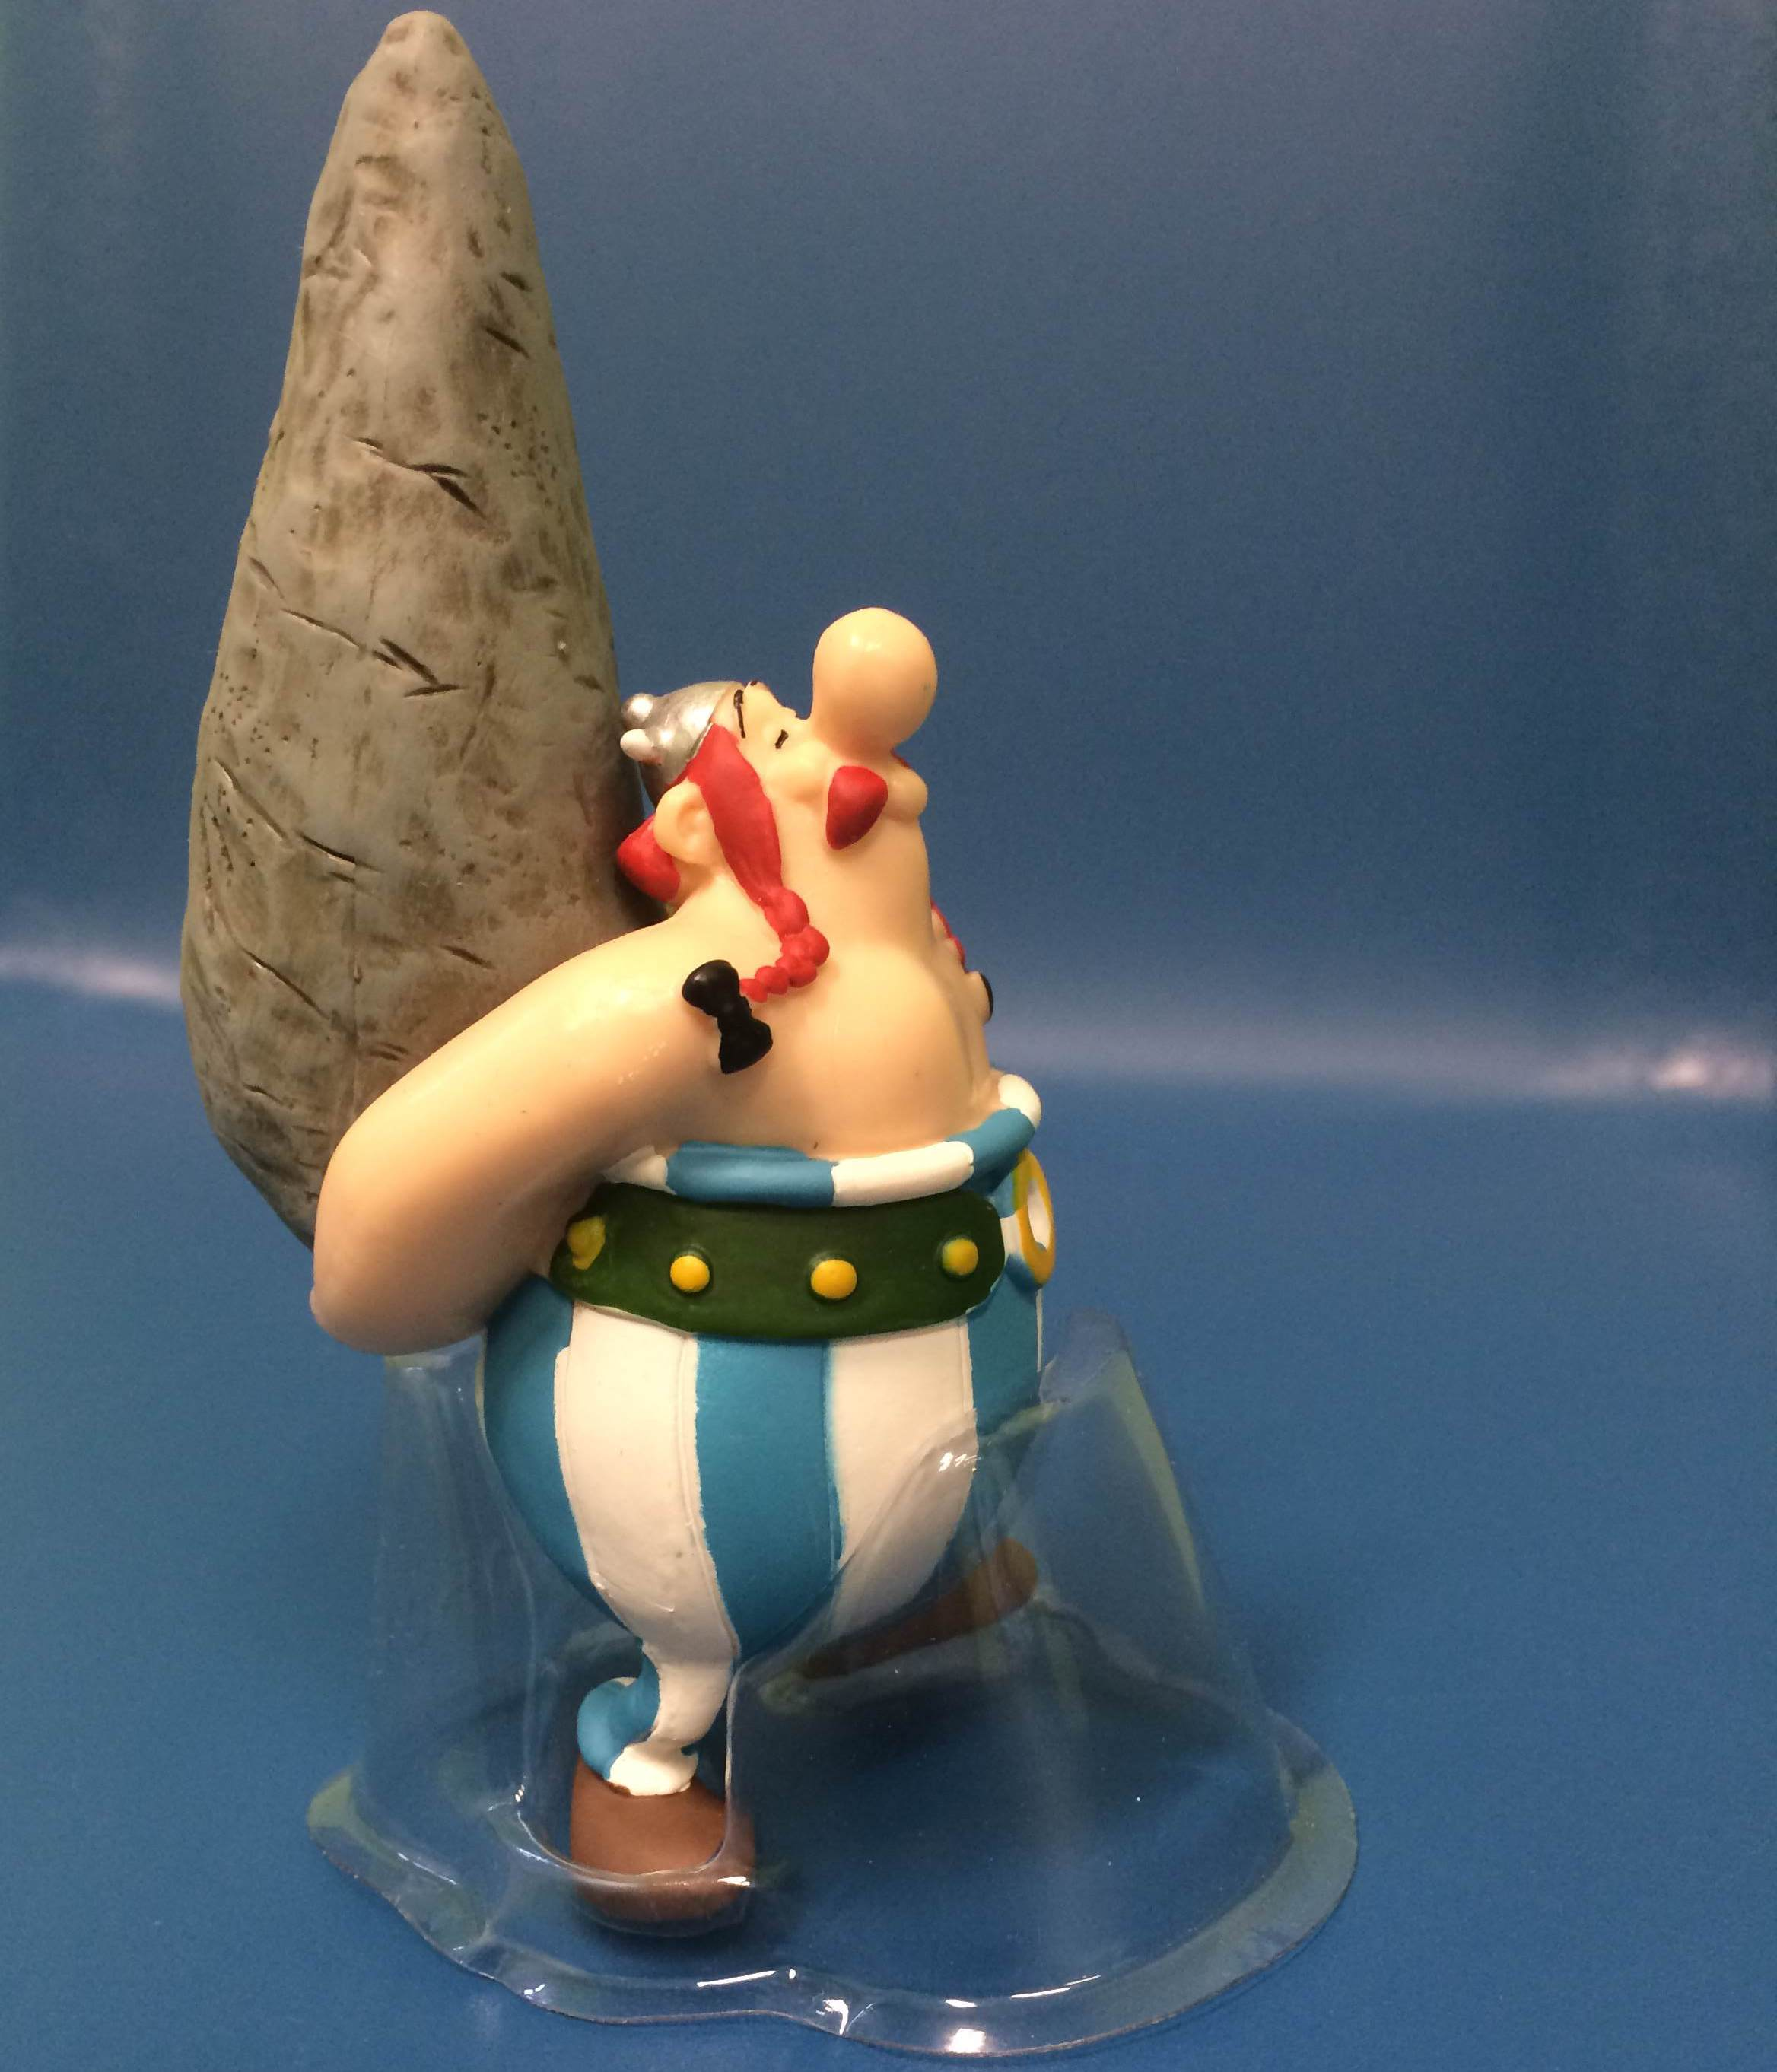
\includegraphics[scale=0.13]{Obelix.jpg}
  \caption{Original}
  \label{fig:sfig1}
\end{subfigure}
\begin{subfigure}{.5\textwidth}
  \centering
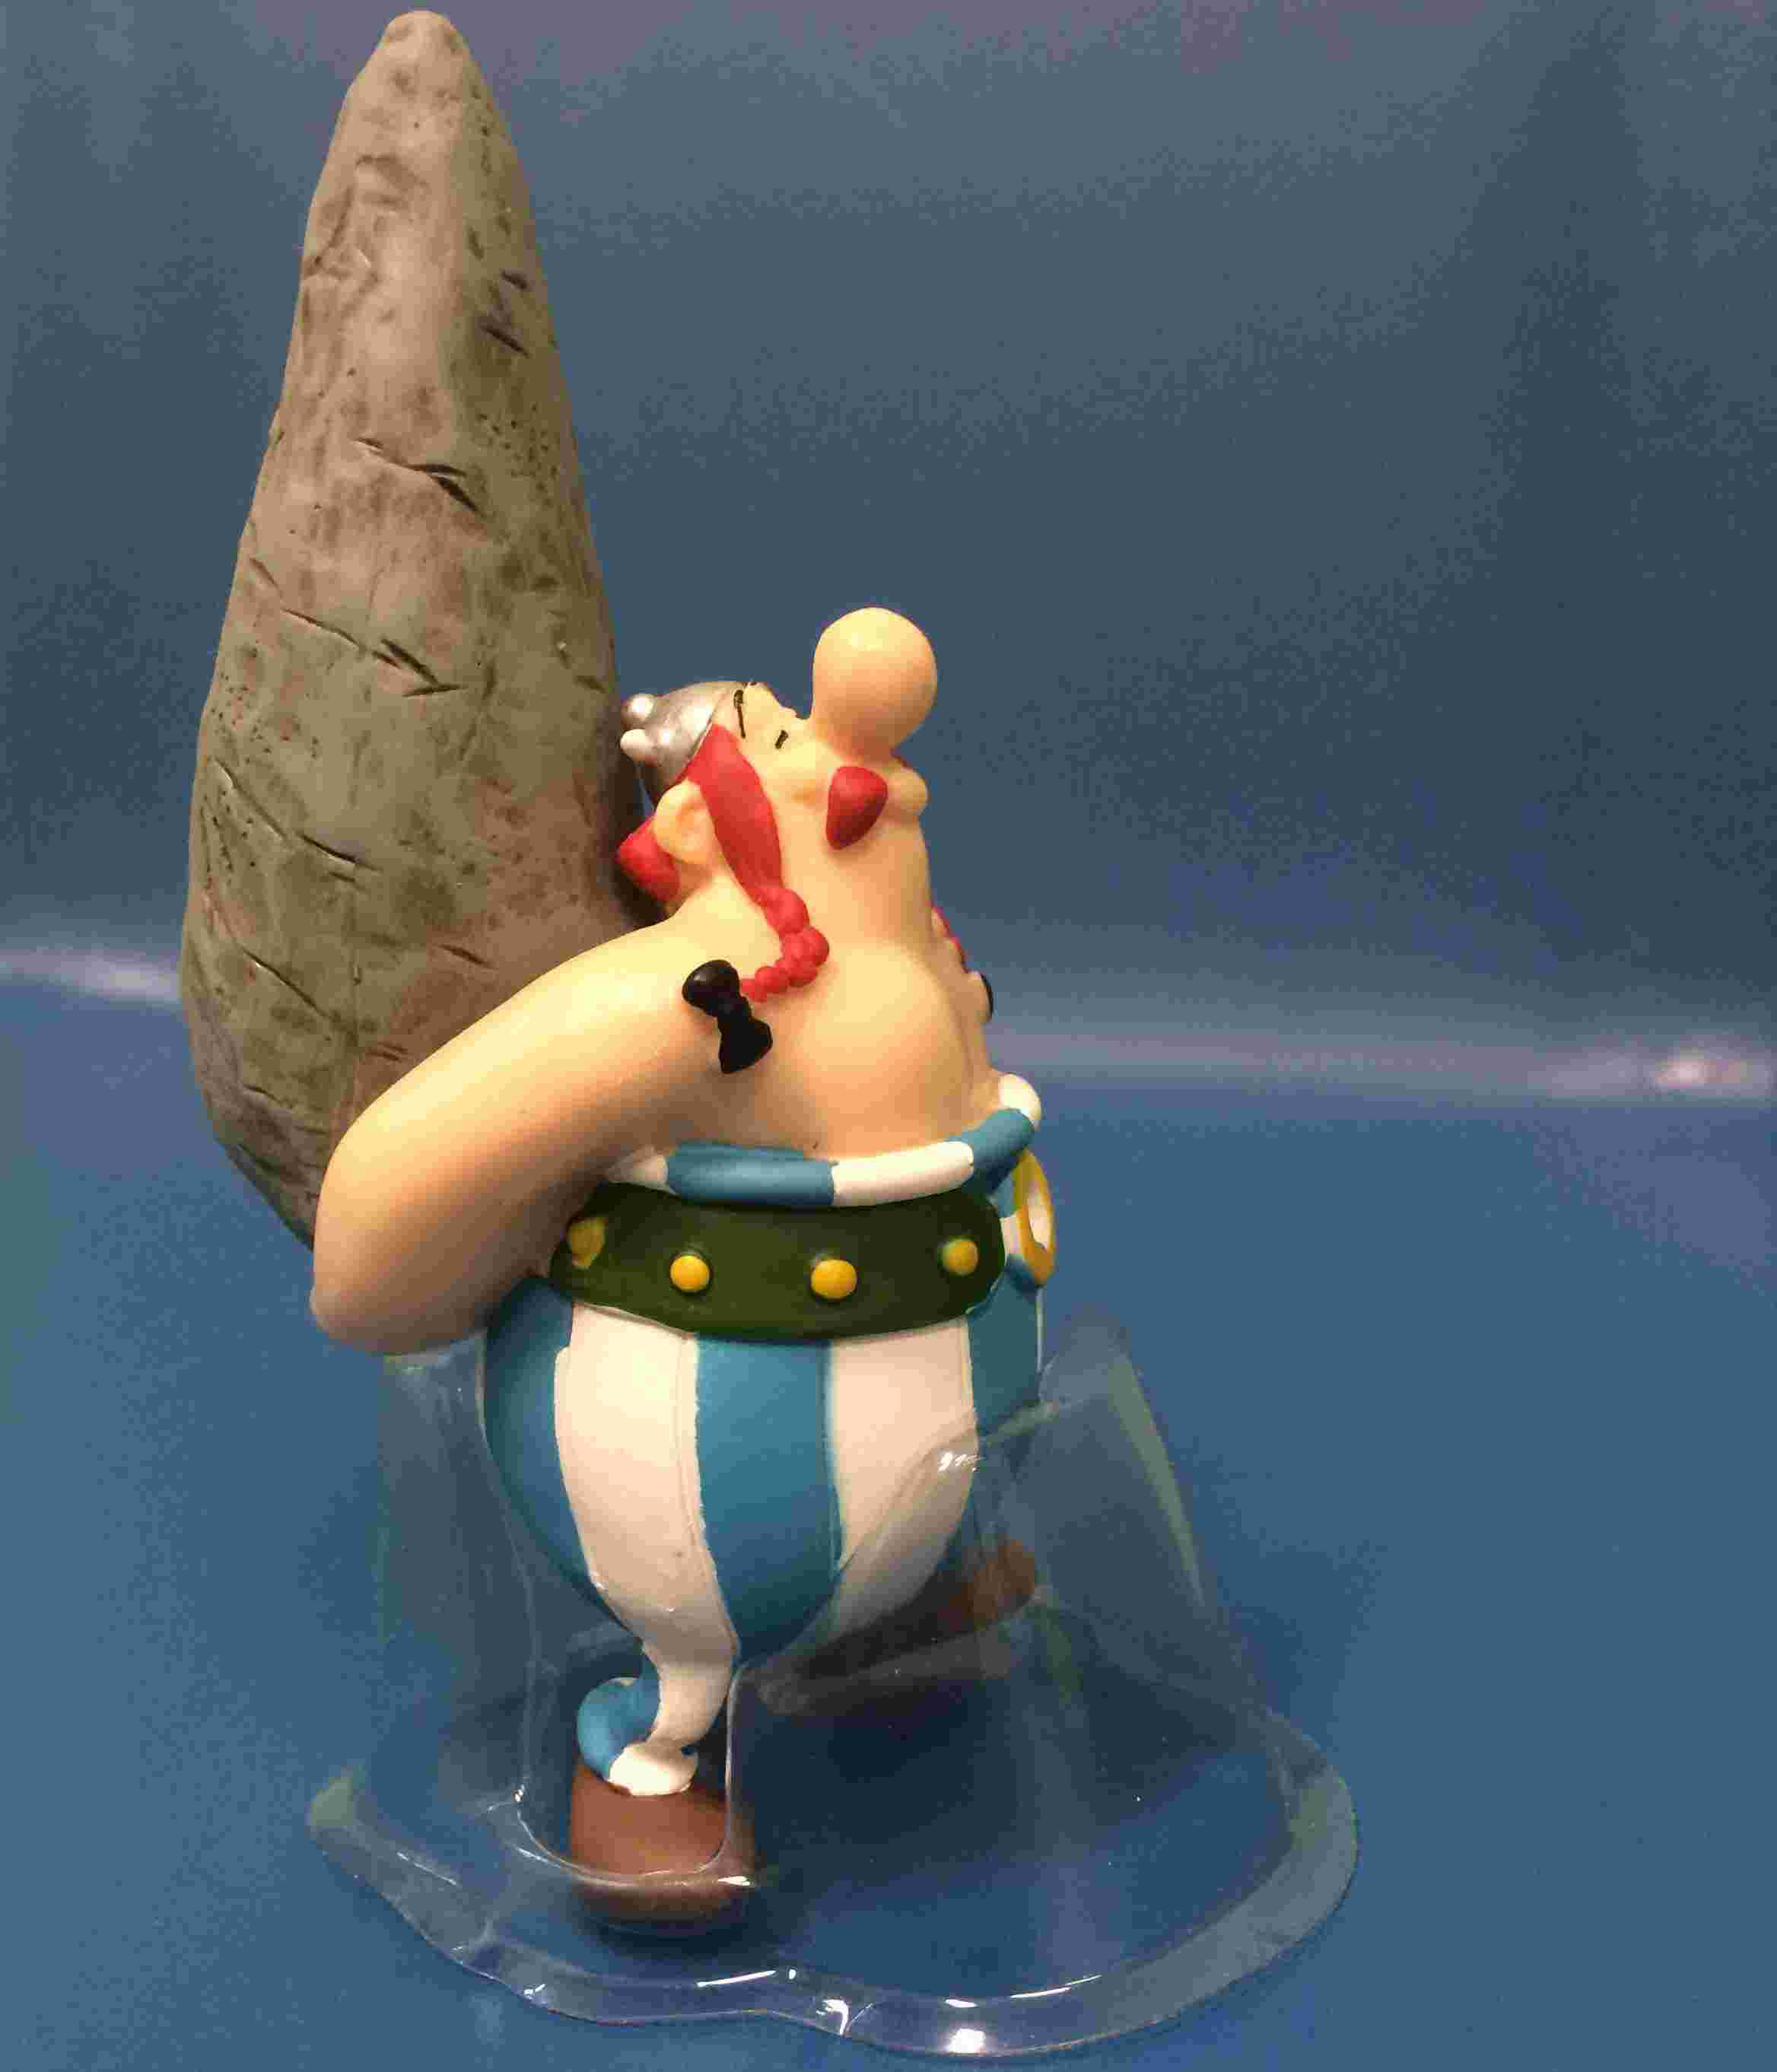
\includegraphics[scale=0.1]{obe_CV2_10.jpg}
  \caption{Opencv compression}
  \label{fig:sfig2}
\end{subfigure}

\begin{subfigure}{.5\textwidth}
\vspace{5mm}
  \centering
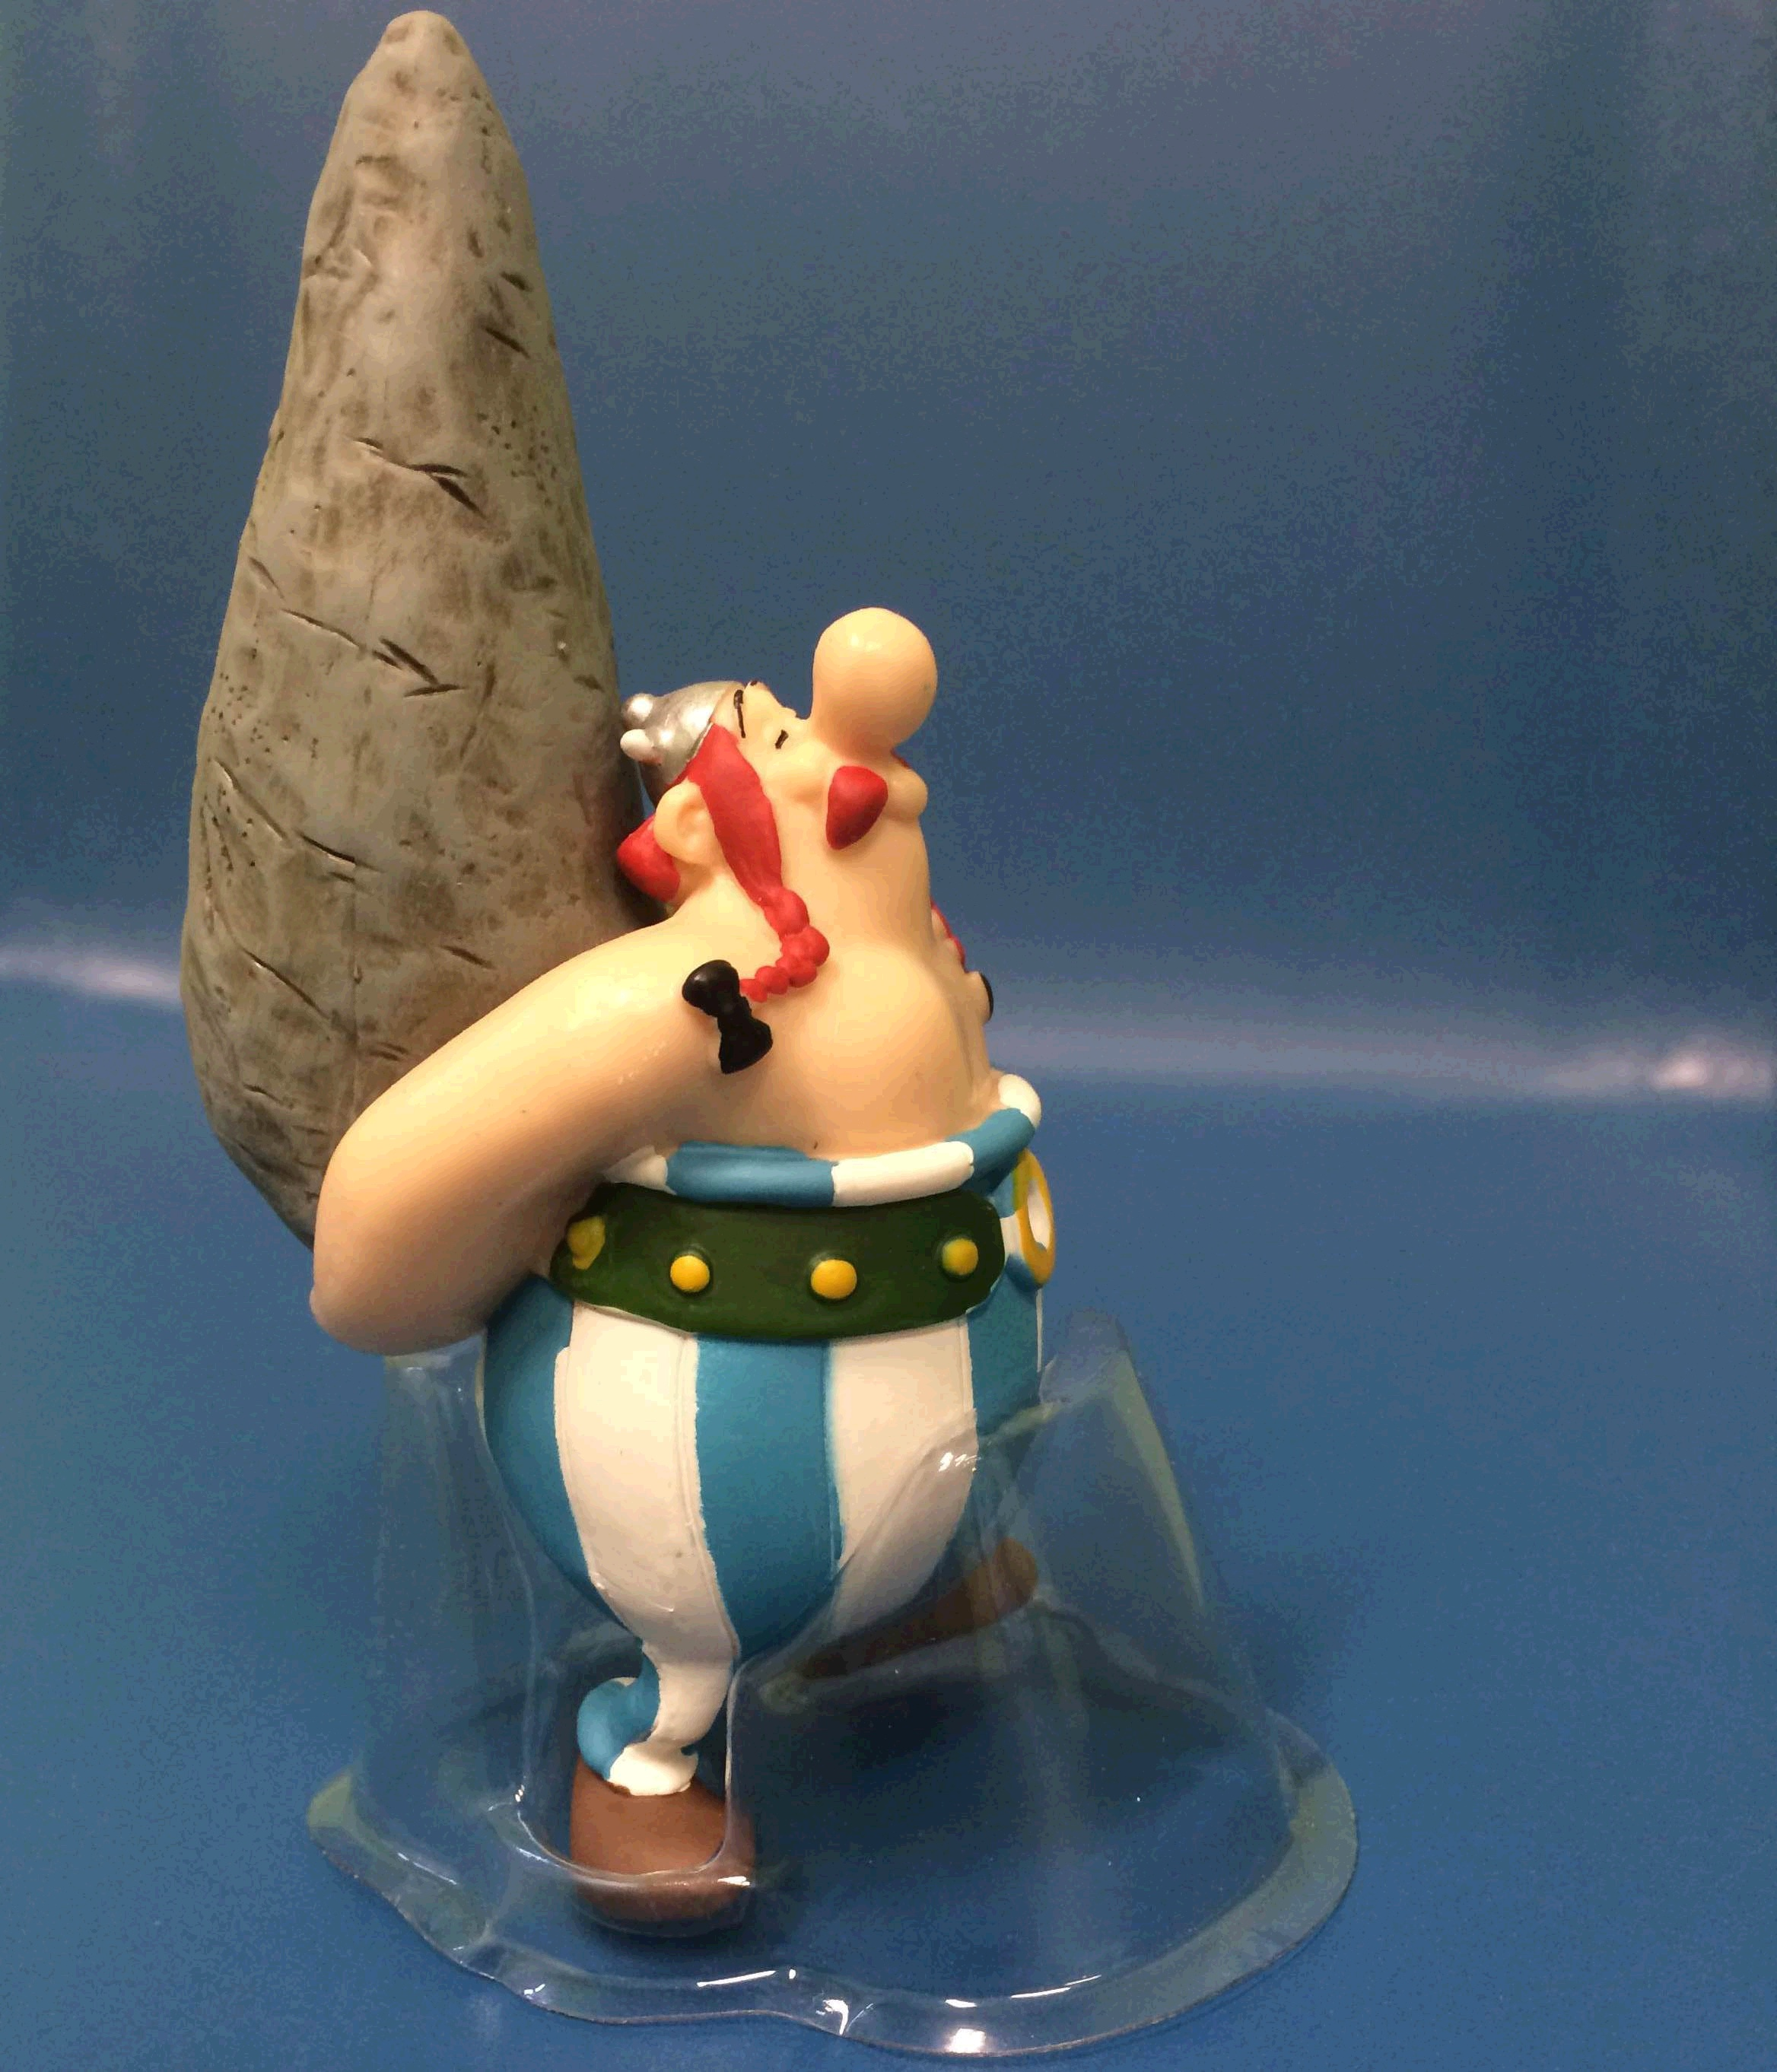
\includegraphics[scale=0.1]{obe_MYWAY_10.jpg}
  \caption{My way Compression}
  \label{fig:sfig1}
  \hspace{5mm}
\end{subfigure}
\caption{Shows compression comparison between original , opencv compression , my way compression}
\end{figure}

To accomplish the previous results I used the following code :
\begin{lstlisting}[language=Python]
import cv2
import numpy as np
from math import floor
def showimg(img):
    cv2.namedWindow("test", cv2.WINDOW_NORMAL)
    img = np.array(img,dtype=float)/float(255)
    cv2.imshow('test',img)
    cv2.resizeWindow('test',600,600)
    cv2.waitKey(0)

def readimg(name):
    return cv2.imread(name)

obe = readimg('Obelix.jpg')

def compressWay1(obe,quality):
    cv2.imwrite('obe_CV2_{}.jpg'.format(quality), obe, [int(cv2.IMWRITE_JPEG_QUALITY), quality])

def compressWay2(obe,quality):
    lvls =floor(quality*255/100)
    step = floor(255/lvls)
    value = floor(step/2)
    print 'levels:{},step:{},value:{},quality:{}'.format(lvls,step,value,quality)
    nm = []
    for i in range(256):
        nm.append(value)
        if i%step==0 and i!=0:
            value+=step
    table = np.array(nm)
    obe = cv2.LUT(obe, table)
    cv2.imwrite('obe_MYWAY_{}.jpg'.format(quality),obe)
    print nm

compressWay1(obe,10)
compressWay2(obe,10)
\end{lstlisting}

\textbf{Note:}All images,.tex,.pdf,.jpg,.py etc.. files exist on \href{https://github.com/aqeel13932/IP/tree/master/hw7}{Github}
\begin{center}
\textbf{E.O.F}
\end{center}
\end{document}